\documentclass{article}
\usepackage{amsmath,amssymb}
\usepackage{fullpage}
\usepackage{mathrsfs}
\usepackage{setspace}
\usepackage{graphicx}
\usepackage{listings}
\renewcommand{\baselinestretch}{1.2}
\pagestyle{empty}

\usepackage{color}
\definecolor{dkgreen}{rgb}{0,0.6,0}
\definecolor{gray}{rgb}{0.5,0.5,0.5}
\definecolor{mauve}{rgb}{0.58,0,0.82}

\lstset{frame=tb,
	language=Matlab,
	aboveskip=3mm,
	belowskip=3mm,
	showstringspaces=false,
	columns=flexible,
	basicstyle={\small\ttfamily},
	numbers=none,
	numberstyle=\tiny\color{gray},
	keywordstyle=\color{blue},
	commentstyle=\color{dkgreen},
	stringstyle=\color{mauve},
	breaklines=true,
	breakatwhitespace=true,
	tabsize=4
}
\begin{document}
\noindent{\bf Homework 1}

\noindent{\bf Jingmin Sun}

\noindent{\bf 661849071}


\begin{enumerate}

\item
Since we need to use the least manipulation as possible, we can use Horner's method:
\begin{align*}
p(x) &= a_7x^7+a_{12}x^{12}+a_{17}x^{17}+a_{22}x^{22}+a_{27}x^{27}\\
&=x^7(a_7+a_{10}x^{5}+a_{17}x^{10}+a_{22}x^{15}+a_{27}x^{20})\\
&=x^7(a_7+x^{5}(a_{10}+a_{15}x^{5}+a_{22}x^{10}+a_{27}x^{15}))\\
&=x^7(a_7+x^{5}(a_{10}+x^{5}(a_{15}+a_{22}x^{5}+a_{27}x^{10})))\\
&=x^7(a_7+x^{5}(a_{10}+x^{5}(a_{15}+x^{5}(a_{22}+a_{27}x^{5}))))\\
\end{align*}

We can easily observe that inside the outer-most parenthesis, it's a formula with typical Horner's method with $x^5$ instead of $x$, so besides $x^5$, there is 4 multiplications and 4 additions, and we need to multiple it as whole with $x^7$, so one more multiplication involved besides $x^7$ and $x^5$.

When we calculate $x^7$, we can use the "storage" method, and on the way, we calculate $x^5$. \begin{align*}
x^2 &= x \cdot x\\
x^3 &= x \cdot x^2\\
x^5 &= x^2 \cdot x^3\\
x^7 &= x^5 \cdot x^2\\ 
\end{align*}
So that there is 4 more multiplications involved to carry out both $x^5$ and $x^7$, thus there are 9 multiplications and 4 additions in total.

\item
Firstly, we can use myPolyEval function to evaluate $p(x)$ as:

\begin{lstlisting}
vec = ones(100,1);
vec(1:2:100) = -1;
a = myPolyEval(1.00001, vec ,99)

a =

  -5.0025e-04
\end{lstlisting}

We can observe that it actually a sum of geometric sequence and $p(x) = \frac{1\cdot(1-(-x)^{100})}{1-(-x)}=\frac{1-x^{100}}{1+x}$, with $x = 1.00001$, so that we can calculate the answer with matlab, and get the answer of \begin{lstlisting}
b = (1-(1.00001)^(100))/(1+1.00001)

b =

  -5.0025e-04
\end{lstlisting}
And the error follows to be:\begin{lstlisting}
error = a - b

error =

  -1.7130e-16
\end{lstlisting}
\item \begin{enumerate}
\item
\begin{align*}
(101.101)_2&= 1\cdot 2^2+0\cdot 2^1+1\cdot 2^{-1} + 0 \cdot 2^{-2}+1\cdot 2^{-3}\\
&=4+0+1+\frac{1}{2}+0+\frac{1}{8}\\
&=5+\frac{5}{8}\\
&=\boxed{\frac{45}{8}}
\end{align*}
\item
$(10.\overline{101})_2:$\\

Let $x =(0.\overline{101})_2 $, $2^3 \cdot x = (101.\overline{101})_2$, so that $(2^3 -1) x = (101)_2= 1\cdot 2^2 +1 =5$, and $x= \frac{5}{7}$ follows.
\begin{align*}
\therefore (10.\overline{101})_2&=(10)_2 + (0.\overline{101})_2\\
&=2+\frac{5}{7}\\
&=\boxed{\frac{19}{7}}
\end{align*}
\end{enumerate}
\item
\begin{enumerate}
\item
In double precision computer arithmetic, the first step is $2^{-51} + 2^{-52}$, which is : $(1.\boxed{10\cdots 0})_2\times 2^{-51}$, and now, we add $2^{-54}$ to it, which is 
\begin{center}
\begin{tabular}{lr}
& $(0.\boxed{000 \cdots 00011}00)_2 \times 2^0$\\
+ &$(0.\boxed{000 \cdots 00000}01)_2 \times 2^0$\\
\hline
& $(0.\boxed{000 \cdots 00011}01)_2 \times 2^0$\\
\end{tabular}
\end{center}
Since the $53^{th}$ bit in the sum is 0, according to the rounding rule, the sum is $(0.\boxed{000 \cdots 00011})_2 \times 2^0$, and now, we add 1 to the sum:
\begin{center}
\begin{tabular}{lr}
& $(1.\boxed{000 \cdots 00000})_2 \times 2^0$\\
+ &$(0.\boxed{000 \cdots 00011})_2 \times 2^0$\\
\hline
& $(1.\boxed{000 \cdots 00011})_2 \times 2^0$\\
\end{tabular}
\end{center}
which is $1+3\times 2^{-52}$, and finally, we subtract 1 and get $3\times 2^{-52}$, which is $3\epsilon_{\text{mach}}$.

And we can check with Matlab:

\begin{lstlisting}
(1+(2^(-51)+2^(-52)+2^(-54)))-1

ans =

   6.6613e-16

ans-3*2^(-52)

ans =

     0

diary off
\end{lstlisting}
\end{enumerate}
\item
Firstly, we need to convert 4.9 and 3.9 into binary form, since $4.9 = 4+ 0.9$, $3.9 = 3+ 0.9$, we need to find the binary form of $3,4,0.9$:

it's easy to observe that $4 = 2^2 = (100)_2$, $3 = 2+1=(11)_2$, and as for 0.9:\begin{align*}
0.9 \times 2 &= 0.8 +1\\
0.8 \times 2 &= 0.6 +1\\
0.6 \times 2 &= 0.2 +1\\
0.2 \times 2 &= 0.4 +0\\
0.4 \times 2 &= 0.8 +0\\
0.8 \times 2 &= 0.6 +1\\
&\cdots
\end{align*}
Thus, $0.9 = 0.1\overline{1100}$

So that $4.9 = (100.1\overline{1100})_2$, $3.9 = (11.1\overline{1100})_2$, in double precision format, \begin{align*}
(100.1\overline{1100})_2 &= (1.\boxed{00111001100\cdots 110011001}\overline{1001})_2 \times 2^2\\
&=(1.\boxed{00111001100\cdots 110011010})_2\times 2^2\\
(11.1\overline{1100})_2 &= (1.\boxed{11110011001\cdots 100110011}\overline{0011})_2 \times 2\\
&=(1.\boxed{11110011001\cdots 100110011})_2\times 2\\
\end{align*}
So that \begin{align*}
4.9 - 3.9 &=(1.\boxed{00111001100\cdots 110011010})_2\times 2^2\\
&-(1.\boxed{11110011001\cdots 100110011})_2\times 2\\
&=(1.\boxed{00111001100\cdots 110011010}0)_2\times 2^2\\
&-(0.\boxed{111110011001\cdots 10011001}1)_2\times 2^2\\
&=(0.\boxed{0100\cdots 00}1 )_2\cdot 2^2\\
&=(1.\boxed{00\cdots 0010})_2\\
&=1+2^{-51}\\
\therefore (4.9 - 3.9 ) -1 &= 2^{-51}
\end{align*}

And we can check with Matlab:\begin{lstlisting}
(4.9 - 3.9) -1

ans =

   4.4409e-16

ans - 2^(-51)

ans =

     0

diary off
\end{lstlisting}

\item
Propose the alternative form of $f(h)$:\begin{align*}
f(h) &= \dfrac{x^4 - (x-h)^4}{h}\\
&=\dfrac{(x^2-(x-h)^2)(x^2+(x-h)^2)}{h}\\
&=\dfrac{x^2-x^2+2xh-h^2}{h}(x^2+(x-h)^2)\\
&=(2x-h)(x^2+(x-h)^2)
\end{align*}
And we can use the following code and get the following data:
\pagebreak
\lstinputlisting[language=Matlab, numbers=left, stepnumber=1, firstline=1,caption={derivative.m},frame=single]{derivative.m}

and the following data:\begin{lstlisting}
 derivative
 T = table(hrt, yr1, yr2, error1, error2)   % Display the table

T =

  15×5 table

     hrt       yr1       yr2        error1        error2  
    ______    ______    ______    __________    __________

       0.1    29.679    29.679      0.072531      0.072531
      0.01    31.761    31.761      0.007475      0.007475
     0.001    31.976    31.976    0.00074975    0.00074975
    0.0001    31.998    31.998    7.4997e-05    7.4998e-05
     1e-05        32        32       7.5e-06       7.5e-06
     1e-06        32        32    7.5009e-07       7.5e-07
     1e-07        32        32    7.4356e-08       7.5e-08
     1e-08        32        32    1.1629e-08       7.5e-09
     1e-09        32        32     8.274e-08       7.5e-10
     1e-10        32        32     8.274e-08       7.5e-11
     1e-11        32        32     8.274e-08       7.5e-12
     1e-12    32.003        32    8.8901e-05    7.5007e-13
     1e-13    31.974        32    0.00079928     7.494e-14
     1e-14    31.974        32    0.00079928    7.5495e-15
     1e-15    35.527        32       0.11022    7.7716e-16

\end{lstlisting}

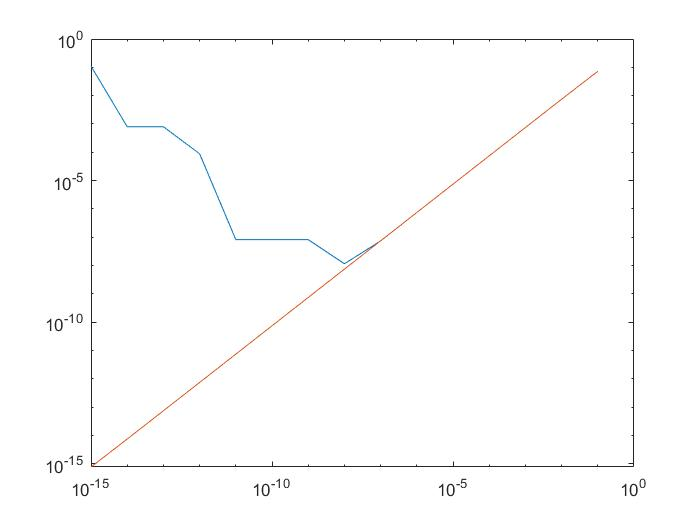
\includegraphics[width=7cm]{question6.jpg}

Since analytically $\lim_{h\rightarrow 0} f(h) = \dfrac{d x^4}{dx} = 4x^3 = 32$ when $x = 2$, and from the figure and the table above, we see that the new method is getting closer to 32 as $h$ approaches 0, but as for the original method, the value of computing value firstly getting closer to 32, but when $h < 10^{-8}$, the error become increasing, and  finally get an error of $0.1102$, this is caused by the subtraction between two similar value ($x^4$ and $(x-h)^4$ as $h \rightarrow 0$). 
\item
\begin{enumerate}
\item
\begin{align*}
b^2 &=(1.234 \times 10^5)^2\\
&= 1.522756 \times 10^{10}\\
\mbox{myfl}(b^2) &=1.523 \times 10^{10}\\
\mbox{myfl}(4a) &=4\\
\mbox{myfl}(4ac)&=\mbox{myfl}(\mbox{myfl}(4a)\times c)\\
&=\mbox{myfl}( 4\cdot 4.567 \times 10^3)\\
&=\mbox{myfl}(1.8268\times 10^4)\\
&=1.827 \times 10^4\\
\end{align*}
\begin{align*}
\mbox{myfl}(b^2-4ac)&=\mbox{myfl}(\mbox{myfl}(b^2)-\mbox{myfl}(4ac))\\
&=\mbox{myfl}(1.523\times 10^{10} - 1.824\times 10^4)\\
&=\mbox{myfl}(1.522998173 \times 10^{10})\\
&=1.523 \times 10^{10}\\
\mbox{myfl}(\sqrt{b^2-4ac})&=\mbox{myfl}(\sqrt{\mbox{myfl}(b^2-4ac)})\\
&=\mbox{myfl}(\sqrt{1.523 \times 10^{10}})\\
&=\mbox{myfl}(1.23409\cdots \times 10^5)\\
&=1.234 \times 10^5\\
\mbox{myfl}(-b )&= -1.234 \times 10^5\\
\mbox{myfl}(-b-\sqrt{b^2-4ac})&=  -1.234 \times 10^5 -1.234 \times 10^5\\&=-2.468 \times 10^5\\
\mbox{myfl}(2a ) &=2\\
\mbox{myfl}\left(\frac{-b-\sqrt{b^2-4ac}}{2a}\right)&=  -1.234 \times 10^5\\
\mbox{myfl}(-b+\sqrt{b^2-4ac})&=  -1.234 \times 10^5 +1.234 \times 10^5\\&=0\\
\mbox{myfl}\left(\frac{-b+\sqrt{b^2-4ac}}{2a}\right)&=  0\\
\therefore \hat{x_1} = -1.234 \times 10^5&,\hat{x_2} =0
\end{align*}

And we can use Matlab to get the "exact" roots and compare the error:
\begin{lstlisting}
a = 1;
b = 1.234*10^5;
c = 4.567*10^3;
x1 = (-b - sqrt(b^2 - 4*a*c))/(2*a);
x2 = (-b + sqrt(b^2 - 4*a*c))/(2*a);
x11 = -1.234*10^5;
x22 = 0;
error1 = abs(x1 -x11)/abs(x1)

error1 =

   2.9992e-07
error2 = abs(x2 -x22)/abs(x2)

error2 =

     1
diary off
\end{lstlisting}
We can observe that $\hat{x_1}$ is approximately accurate, but $\hat{x_2}$ is not so accurate.

\item
Since $\hat{x_2}$ is the one with larger error, we can use \begin{align*}
x_2 &=\dfrac{-b+\sqrt{b^2 - 4ac}}{2a}\\
&=\dfrac{-2c}{b+\sqrt{b^2-4ac}}\\
\end{align*}
Since $\mbox{myfl}(b) = 1.234\times 10^5$,  $\mbox{myfl}(\sqrt{b^2-4ac}) = 1.234\times 10^5$, so that $\mbox{myfl}(b+\sqrt{b^2-4ac}) = 2.468\times 10^5$.

Since $\mbox{myfl}(-2c) = \mbox{myfl}(-2\times 4.567\times 10^3) = -9.134\times 10^3$,
\begin{align*}
\therefore \dfrac{\mbox{myfl}(-2c)}{\mbox{myfl}(b+\sqrt{b^2-4ac})}&=\frac{-9.134\times 10^3}{2.468\times 10^5}\\
&=-3.7009\cdots \times 10^{-2}\\
\therefore \hat{x_2}&=-3.701\times 10^{-2}
\end{align*}
And we can check with Matlab that the error reduces a lot:

\begin{lstlisting}
x2 = (-2*c)/(b+sqrt(b^2-4*a*c));
x22 = -3.701 *10^(-2);
error2 = abs(x2 -x22)/abs(x2)

error2 =

   7.1448e-06

diary off

\end{lstlisting}
\end{enumerate}
\end{enumerate}
\end{document}